%\documentclass{standalone}
\documentclass[16pt]{article}
\usepackage{tikz}
\usetikzlibrary{decorations.pathreplacing}
\usepackage{colortbl}
%\documentclass{minimal}
%\usepackage[active,tightpage,displaymath]{preview}
%\documentclass{article}
\usepackage{blkarray}
\usepackage{amsmath}
\pagestyle{empty}
\usepackage[paperheight=16cm,paperwidth=33cm]{geometry}
%\usepackage[absolute]{textpos}

\definecolor{c1}{RGB}{102,194,165}
\definecolor{c2}{RGB}{252,141,98}
\definecolor{c3}{RGB}{141,160,203}
\definecolor{c4}{RGB}{231,138,195}

\newcolumntype{a}{>{\columncolor{LightYellow}}l}
\newcolumntype{b}{>{\columncolor{LightYellow}}c}
\newcolumntype{d}{>{\columncolor{LightGrey}}l}
\newcolumntype{e}{>{\columncolor{LightGrey}}c}

\begin{document}
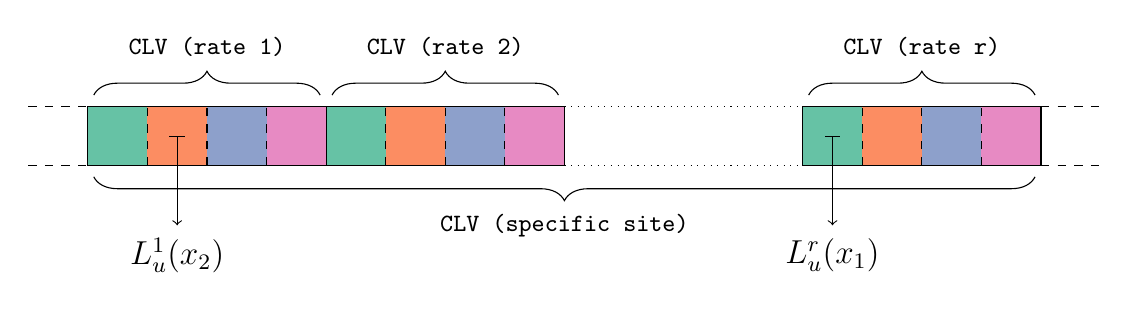
\begin{tikzpicture}[font=\small]

%%% First quadruple of colors 
\fill[c1] (0ex,5ex) rectangle (5ex,0ex);
\fill[c2] (5ex,5ex) rectangle (10ex,0ex);
\fill[c3] (10ex,5ex) rectangle (15ex,0ex);
\fill[c4] (15ex,5ex) rectangle (20ex,0ex);

%%% Second quadruple of colors 
\fill[c1] (20ex,5ex) rectangle (25ex,0ex);
\fill[c2] (25ex,5ex) rectangle (30ex,0ex);
\fill[c3] (30ex,5ex) rectangle (35ex,0ex);
\fill[c4] (35ex,5ex) rectangle (40ex,0ex);

%%% Fourth quadruple of colors 
\fill[c1] (60ex,5ex) rectangle (65ex,0ex);
\fill[c2] (65ex,5ex) rectangle (70ex,0ex);
\fill[c3] (70ex,5ex) rectangle (75ex,0ex);
\fill[c4] (75ex,5ex) rectangle (80ex,0ex);

\draw (0ex,0ex) -- (40ex,0ex) -- (40ex,5ex) -- (0ex,5ex) -- (0ex,0ex);
\draw (60ex,0ex) -- (80ex,0ex) -- (80ex,5ex) -- (60ex,5ex) -- (60ex,0ex);

\draw[dotted] (40ex,0ex) -- (60ex,0ex);
\draw[dotted] (40ex,5ex) -- (60ex,5ex);

\draw (20ex,0ex) -- (20ex,5ex);
\draw[dashed] (5ex,0ex) -- (5ex,5ex);
\draw[dashed] (10ex,0ex) -- (10ex,5ex);
\draw[dashed] (15ex,0ex) -- (15ex,5ex);

\draw (40ex,0ex) -- (40ex,5ex);
\draw[dashed] (25ex,0ex) -- (25ex,5ex);
\draw[dashed] (30ex,0ex) -- (30ex,5ex);
\draw[dashed] (35ex,0ex) -- (35ex,5ex);

\draw (80ex,0ex) -- (80ex,5ex);
\draw[dashed] (65ex,0ex) -- (65ex,5ex);
\draw[dashed] (70ex,0ex) -- (70ex,5ex);
\draw[dashed] (75ex,0ex) -- (75ex,5ex);

\draw[decorate,decoration={brace,amplitude=2ex,raise=4pt},yshift=0pt] (0.5ex, 5ex) -- (19.5ex,5ex);
\draw[decorate,decoration={brace,amplitude=2ex,raise=4pt},yshift=0pt] (20.5ex, 5ex) -- (39.5ex,5ex);
\draw[decorate,decoration={brace,amplitude=2ex,raise=4pt},yshift=0pt] (60.5ex, 5ex) -- (79.5ex,5ex);
\node at (10ex,10ex) {\tt CLV (rate 1)};
\node at (30ex,10ex) {\tt CLV (rate 2)};
\node at (70ex,10ex) {\tt CLV (rate r)};
\draw[decorate,decoration={brace,amplitude=2ex,mirror,raise=4pt},yshift=0pt] (0.5ex, 0ex) -- (79.5ex,0ex);
\node at (40ex,-5ex) {\tt CLV (specific site)};

\draw[<-|] (7.5ex,-5ex) -- (7.5ex,2.5ex);
\node at (7.5ex,-7.5ex) {\large $L^{1}_u(x_2)$};

\draw[<-|] (62.5ex,-5ex) -- (62.5ex,2.5ex);
\node at (62.5ex,-7.5ex) {\large $L^{r}_u(x_1)$};

\draw[dashed] (-5ex,0ex) -- (0ex,0ex);
\draw[dashed] (-5ex,5ex) -- (0ex,5ex);
\draw[dashed] (80ex,5ex) -- (85ex,5ex);
\draw[dashed] (80ex,0ex) -- (85ex,0ex);
\end{tikzpicture}
\end{document}
